%% appendix.tex
%%

%% ==============================
\Appendix
\label{ch:Appendix}
%% ==============================
\section{Available Quality of Service Profiles for the Distributed Topics}\label{sec:app-qos}
An explanation of the profiles can be found here: \href{https://docs.ros.org/en/rolling/Concepts/Intermediate/About-Quality-of-Service-Settings.html}{QoS explanation}.
\subsubsection*{Sensor Profile - Used for the Evaluation}
\lstset{language=C++,basicstyle=\scriptsize}
\begin{lstlisting}[caption=Sensor data profile.,label=ca_code_qos_sensor_profile]
static const rmw_qos_profile_t rmw_qos_profile_sensor_data = {
  RMW_QOS_POLICY_HISTORY_KEEP_LAST,
  5,
  RMW_QOS_POLICY_RELIABILITY_BEST_EFFORT,
  RMW_QOS_POLICY_DURABILITY_VOLATILE,
  RMW_QOS_DEADLINE_DEFAULT,
  RMW_QOS_LIFESPAN_DEFAULT,
  RMW_QOS_POLICY_LIVELINESS_SYSTEM_DEFAULT,
  RMW_QOS_LIVELINESS_LEASE_DURATION_DEFAULT,
  false};
\end{lstlisting}
\subsubsection*{Sensor Profile One}
\begin{lstlisting}[caption=Sensor data profile with history of 1.,label=ca_code_qos_sensor_1_profile]
static const rmw_qos_profile_t rmw_qos_profile_sensor_data_1 = {
  RMW_QOS_POLICY_HISTORY_KEEP_LAST,
  1,
  RMW_QOS_POLICY_RELIABILITY_BEST_EFFORT,
  RMW_QOS_POLICY_DURABILITY_VOLATILE,
  RMW_QOS_DEADLINE_DEFAULT,
  RMW_QOS_LIFESPAN_DEFAULT,
  RMW_QOS_POLICY_LIVELINESS_SYSTEM_DEFAULT,
  RMW_QOS_LIVELINESS_LEASE_DURATION_DEFAULT,
  false};
\end{lstlisting}
\subsubsection*{Sensor Profile 100}
\begin{lstlisting}[caption=Sensor data profile with history of 100.,label=ca_code_qos_sensor_1_profile]
static const rmw_qos_profile_t rmw_qos_profile_sensor_data_100 = {
  RMW_QOS_POLICY_HISTORY_KEEP_LAST,
  100,
  RMW_QOS_POLICY_RELIABILITY_BEST_EFFORT,
  RMW_QOS_POLICY_DURABILITY_VOLATILE,
  RMW_QOS_DEADLINE_DEFAULT,
  RMW_QOS_LIFESPAN_DEFAULT,
  RMW_QOS_POLICY_LIVELINESS_SYSTEM_DEFAULT,
  RMW_QOS_LIVELINESS_LEASE_DURATION_DEFAULT,
  false};
\end{lstlisting}
\subsubsection*{Reliable Profile - Used for the Evaluation}
\begin{lstlisting}[caption=Reliable profile.,label=ca_code_qos_reliable]
static const rmw_qos_profile_t rmw_qos_profile_reliable = {
  RMW_QOS_POLICY_HISTORY_KEEP_LAST,
  1,
  RMW_QOS_POLICY_RELIABILITY_RELIABLE,
  RMW_QOS_POLICY_DURABILITY_VOLATILE,
  RMW_QOS_DEADLINE_DEFAULT,
  RMW_QOS_LIFESPAN_DEFAULT,
  RMW_QOS_POLICY_LIVELINESS_SYSTEM_DEFAULT,
  RMW_QOS_LIVELINESS_LEASE_DURATION_DEFAULT,
  false};
\end{lstlisting}
\subsubsection*{Sensor Profile One}
\begin{lstlisting}[caption=System default profile.,label=ca_code_qos_system_default]
static const rmw_qos_profile_t rmw_qos_profile_system_default = {
  RMW_QOS_POLICY_HISTORY_SYSTEM_DEFAULT,
  RMW_QOS_POLICY_DEPTH_SYSTEM_DEFAULT,
  RMW_QOS_POLICY_RELIABILITY_SYSTEM_DEFAULT,
  RMW_QOS_POLICY_DURABILITY_SYSTEM_DEFAULT,
  RMW_QOS_DEADLINE_DEFAULT,
  RMW_QOS_LIFESPAN_DEFAULT,
  RMW_QOS_POLICY_LIVELINESS_SYSTEM_DEFAULT,
  RMW_QOS_LIVELINESS_LEASE_DURATION_DEFAULT,
  false};
\end{lstlisting}

\section{Platform Used for the Evaluation}
\begin{figure}[htbp]
	\centering
	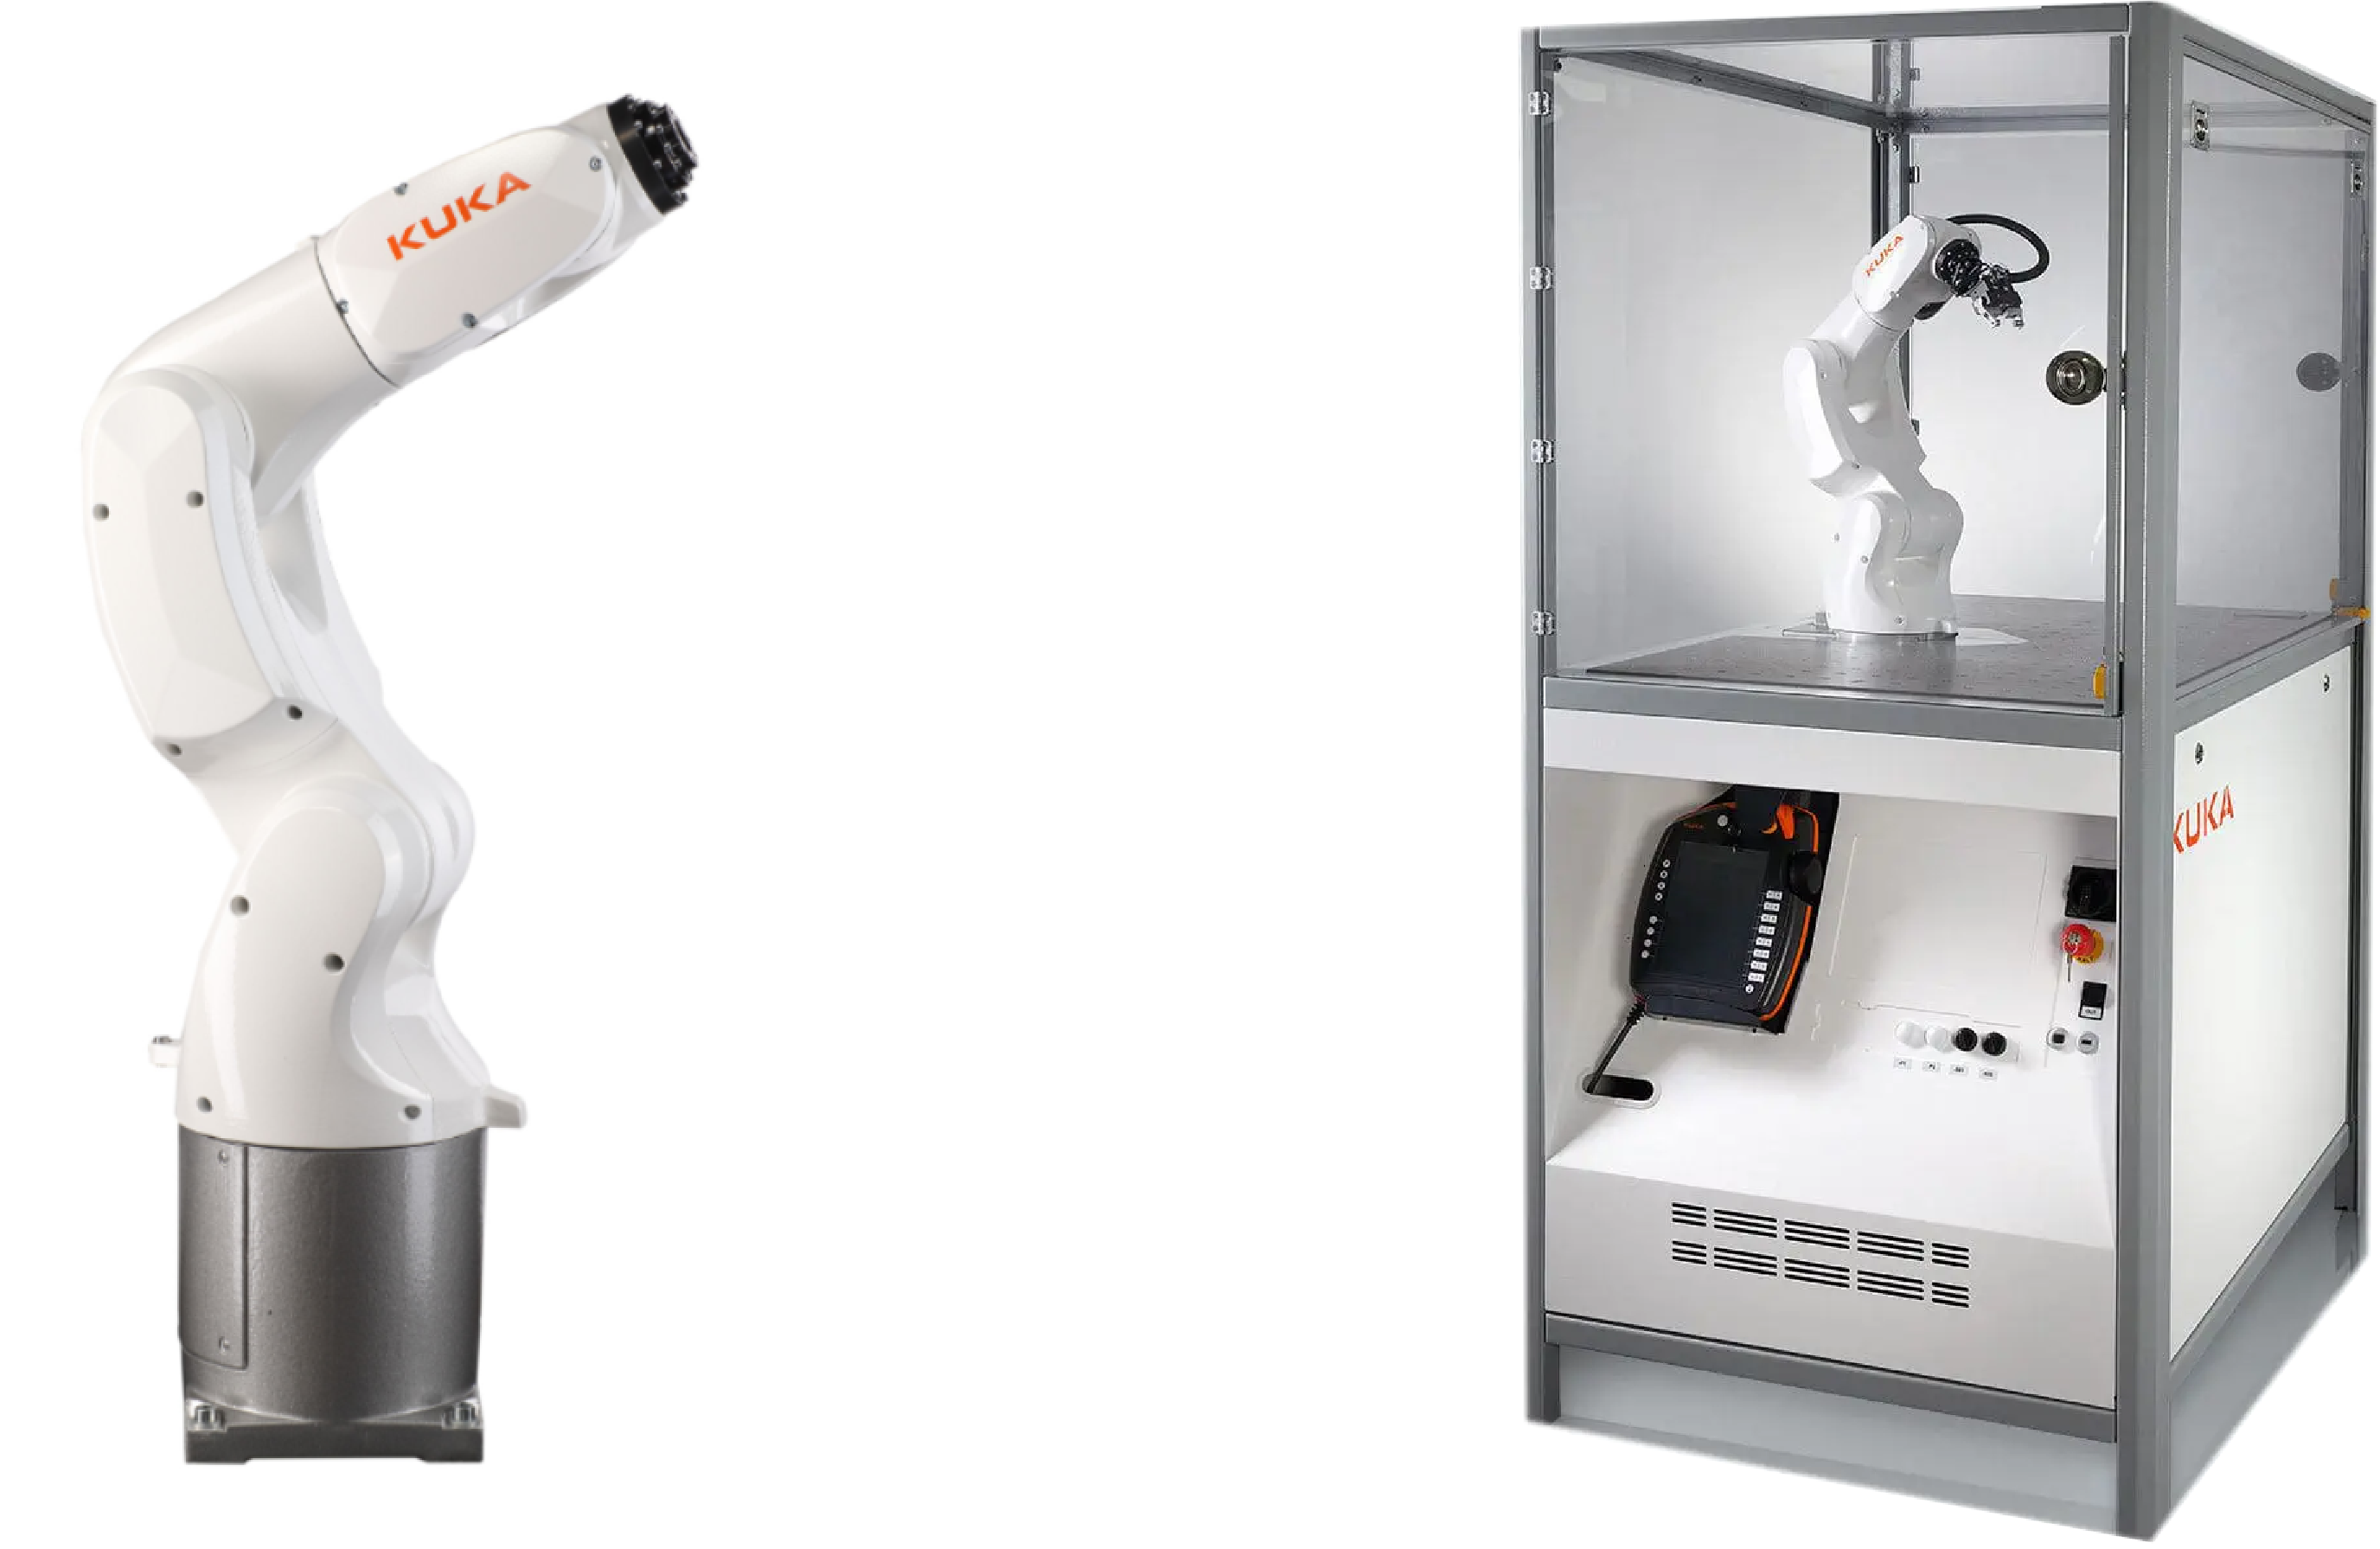
\includegraphics[width=1\textwidth]{Figures/c3/robot_and_cell.pdf}
	\caption{On the left, the KUKA KR 3 R540 is shown. Picture taken from \cite{noauthor_kuka_kr_3_agiluspdf_nodate}. On the right the \textit{ready2\_educate} platform is depicted in which the robots are mounted. Picture from \cite{noauthor_ready2_educate_nodate}.}
	\label{ca_fig_r2c_mr_is}
\end{figure}
